%----------------------------------------------------------------------------------------
%	PACKAGES AND THEMES
%----------------------------------------------------------------------------------------

\documentclass{beamer}

\mode<presentation> {

\usetheme{Madrid}

}


\usepackage{graphicx} % Allows including images
\usepackage{booktabs} % Allows the use of \toprule, \midrule and \bottomrule in tables

\usepackage[normalem]{ulem} % strike text
\usepackage{verbatim}

%%% Работа с русским языком
\usepackage[T2A]{fontenc}			% кодировка
\usepackage[LGR,T1]{fontenc}
\usepackage[utf8]{inputenc}			% кодировка исходного текста
\usepackage[english, russian]{babel}	% локализация и переносы

%%% Работа с картинками
\setlength\fboxsep{3pt} % Отступ рамки \fbox{} от рисунка
\setlength\fboxrule{1pt} % Толщина линий рамки \fbox{}
\usepackage{wrapfig} % Обтекание рисунков текстом

%%% Оформление стихов
\usepackage{verse}

\usepackage{philex}

%%% Зачёркивания
\usepackage{ulem}

%%% Параллельные тексты
\usepackage{parallel}


\AtBeginSection[]
{
  \begin{frame}
    \frametitle{Содержание}
    \tableofcontents[currentsection]
  \end{frame}
}


%%%%%%%%%%%%%%%%%%%%%%%%%%%%%%  LaTeX commands.
\DeclareRobustCommand{\greektext}{%
  \fontencoding{LGR}\selectfont\def\encodingdefault{LGR}}
\DeclareRobustCommand{\textgreek}[1]{\leavevmode{\greektext #1}}
\DeclareFontEncoding{LGR}{}{}
\DeclareTextSymbol{\~}{LGR}{126}


%----------------------------------------------------------------------------------------
%	TITLE PAGE
%----------------------------------------------------------------------------------------

\title[Занятие 4]{Формальный анализ стиха. Занятие 4} % The short title appears at the bottom of every slide, the full title is only on the title page

\author{Борис Орехов} % Your name
\institute[НИУ ВШЭ] % Your institution as it will appear on the bottom of every slide, may be shorthand to save space
{
НИУ Высшая школа экономики \\ % Your institution for the title page
\medskip
\textit{nevmenandr@gmail.com} % Your email address
}
\date{29 сентября 2015} % Date, can be changed to a custom date

\begin{document}

\begin{frame}
\titlepage % Print the title page as the first slide
\end{frame}



\begin{frame}
\frametitle{Содержание}  % Table of contents slide, comment this block out to remove it
\tableofcontents % Throughout your presentation, if you choose to use \section{} and \subsection{} commands, these will automatically be printed on this slide as an overview of your presentation
\end{frame}

%----------------------------------------------------------------------------------------
%	PRESENTATION SLIDES
%----------------------------------------------------------------------------------------



%------------------------------------------------
\section{Вспоминаем системы стихосложения}\label{sec:sys} % Sections can be created in order to organize your presentation into discrete blocks, all sections and subsections are automatically printed in the table of contents as an overview of the talk
%------------------------------------------------



\begin{frame}
\frametitle{В каких системах эти примеры?}

\lb{ex1}{
\begin{verse}
Что так смутен, дружок мой? Щеки внутрь опали,\\
Бледен, и глаза красны, как бы ночь не спали?\\
Задумчив, как тот, что, чин патриарш достати\\
Ища, конный свой завод раздарил некстати?
\end{verse}
}

\lb{ex2}{
\begin{verse}
Преданье есть: во дни царя Гороха\\
Расчищен был весь мир, как огород,\\
И без хлопот, и без переполоха\\
Везде росли рожь, овощи и плод.
\end{verse}
}

\lb{ex3}{
\begin{verse}
Гражданин фининспектор! Простите за ~беспокойство.\\
Спасибо\dots не тревожтесь\dots я постою\dots\\
У меня к~вам дело деликатного свойства:\\
о~месте поэта в~рабочем строю.
\end{verse}
}

\end{frame}


\section{Реформа русского стихосложения}\label{sec:sys}

%------------------------------------------------

\begin{frame}
\frametitle{Основные теоретические тексты реформы}

\begin{itemize}
\item В.",К.",Тредиаковский «Новый и краткий способ к~сложению российских стихов с~определениями до~сего надлежащих званий» (1735);
\item М.",В.",Ломоносов  «Письмо о~правилах Российского стихотворства» (1739);
\item А.",Д.",Кантемир «Письмо Харитона Макентина к~приятелю о~сложении стихов русских» (1743).
\end{itemize}

\end{frame}

%------------------------------------------------

\begin{frame}
\frametitle{Василий Кириллович Тредиакоовский (Тредьяковский) }
\begin{flushleft}
22~февраля (5~марта) 1703~года, Астрахань\,--\,
6~августа 1769~года, Санкт"=Петербург
\end{flushleft}

\begin{flushleft}
Теоретик и~усердный практик русского стиха XVIII~века. Постоянный объект насмешек современников и~ближайших потомков, но~оценённый позднее как~первопроходец.
\end{flushleft}

\end{frame}

%

\begin{frame}
\frametitle{Этимологии Тредиаковского}

\begin{itemize}
\item скифы $ \leftarrow $ скитания, свободное прехождения с~места на~место
\item амазонки (амазоны) $ \leftarrow $ омужоны, т.~е. «омуженные», мужественные жены
\item Каледония $ \leftarrow $ хлад, Хладония
\item Италия $ \leftarrow $ удаль, Удалия
\item Сицилия $ \leftarrow $ Сечелия, «как~отсеченная от~Италии»
\item Британия $ \leftarrow $ Пристания, Бродания или~Братания
\item сарматы $ \leftarrow $ Цар-меты, т.~е. искусные метатели, ср.~царь"=колокол, царь"=девица
\end{itemize}

\end{frame}

%

\begin{frame}
\frametitle{Плач одного любовника, разлучившегося с своей милой, которую он видел во сне}

\begin{verse}
Ах! невозможно сердцу пробыть без печали,\\
Хоть уж и глаза мои плакать перестали:\\
Ибо сердечна друга не могу забыти,\\
Без которого всегда принужден я быти.

Но, принужден судьбою или непременной,\\
И от всея вечности тако положенной,\\
Или насильно волей во всем нерассудной,\\
И в порыве склониться на иное трудной.

\end{verse}
<1730>
\end{frame}

\begin{frame}
\frametitle{Элегия I}

\begin{verse}
Не возможно сердцу, ах! не иметь печали;\\
Очи такожде еще плакать не престали:\\
Друга милого весьма не могу забыти,\\
Без которого теперь надлежит мне жити.\\
Вижу, ах! что надлежит, чрез судьбу жестоку,\\
Язву сердца внутрь всего толь питать глубоку:\\
С Илидарою навек я уж разлучился\\
И в последние тогда весь в слезах простился;
\end{verse}
1735
\end{frame}

%------------------------------------------------


\begin{frame}
\frametitle{Стихи похвальные России}

Система стихосложения: квантитативная, метрическая

\begin{verse}
Начну на флейте стихи печальны,\\
Зря на Россию чрез страны дальны:\\
Ибо все днесь мне ее доброты\\
Мыслить умом есть много охоты.

Россия мати! свет мой безмерный!\\
Позволь то, чадо прошу твой верный,\\
Ах, как сидишь ты на троне красно!\\
Небо российску ты солнце ясно!

\end{verse}
1728

\end{frame}

%------------------------------------------------

\begin{frame}
\frametitle{Михаил (Михайло) Васильевич Ломоносов}

\begin{flushleft}
8 (19) ноября 1711, деревня Мишанинская — 4 (15) апреля 1765, Санкт-Петербург
\end{flushleft}

\begin{flushleft}
Популяризатор науки, мысливший своим главным занятием горное дело, получил положение при дворе благодаря торжественным одам, сочинявшимся каждый год на день восшествия на престол императрицы Елизаветы Петровны. 
\end{flushleft}

\end{frame}

%------------------------------------------------


\begin{frame}
\frametitle{Ода на взятие Хотина}
\begin{center}
\textbf{Ода блаженныя памяти государыне императрице Анне~Иоанновне на~победу над турками и татарами и~на~взятие Хотина 1739~года}
\end{center}

\begin{verse}
Восторг внезапный ум пленил,\\
Ведет на верьх горы высокой,\\
Где ветр в лесах шуметь забыл;\\
В долине тишина глубокой.\\
Внимая нечто, ключ молчит,\\
Которой завсегда журчит\\
И с шумом в низ с холмов стремится.\\
Лавровы вьются там венцы,\\
Там слух спешит во все концы;\\
Далече дым в полях курится. <...>
\end{verse}
\end{frame}

%------------------------------------------------

\begin{frame}
\frametitle{В.",Ходасевич <<Не ямбом ли четырехстопным\dots>>}

\begin{verse}
Из памяти изгрызли годы,\\
За что и кто в Хотине пал,\\
Но первый звук Хотинской оды\\
Нам первым криком жизни стал.
\end{verse}

1938
\end{frame}

%------------------------------------------------

\begin{frame}
\frametitle{Хотинская крепость}
\begin{center}
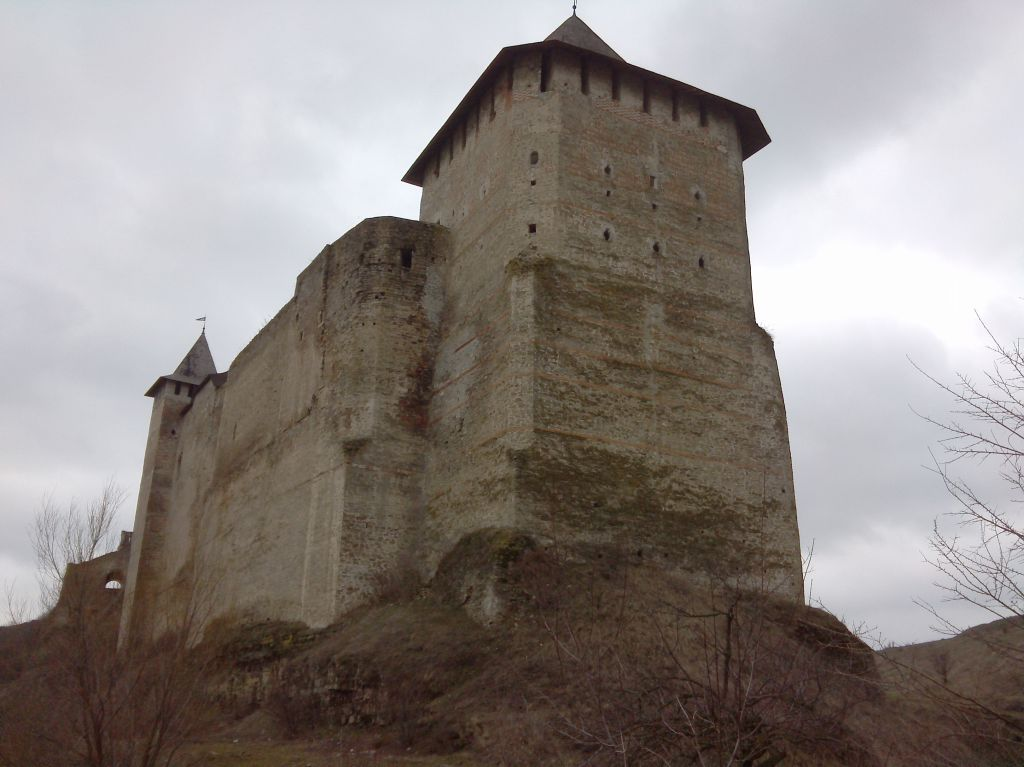
\includegraphics[width=0.8\textwidth]{Xotin.jpg}
\end{center}

\end{frame}

%------------------------------------------------


\begin{frame}
\frametitle{25 ноября 1741 г.}
До (лето 1741):

\begin{verse}
Цел\'{у}ю Р\'{у}чки, чт\'{о} к держ\'{а}ве\\
Прир\'{о}да м\'{у}дра в св\'{е}т дал\'{а},\\
Кот\'{о}ры б\'{у}дут в гр\'{о}мкой сл\'{а}ве\\
Меч\'{е}м страш\'{и}ть и гн\'{а}ть враг\'{а}.\\
От т\'{е}плых \'{у}ж брег\'{о}в Ази\'{и}йских\\
Всел\'{е}нной ч\'{а}сть до в\'{о}д Балт\'{и}йских\\
В объ\'{я}тьи В\'{а}шем вс\'{я} ле\'{ж}ит.\\
Лишь т\'{о}лько П\'{е}рстик В\'{а}ш погн\'{е}тся,\\
Нар\'{о}д бесч\'{и}слен вдр\'{у}г збер\'{е}тся,\\
Гот\'{о}в итт\'{и}, куд\'{а} вел\'{и}т.
\end{verse}
\end{frame}

\begin{frame}
\frametitle{25 ноября 1741 г.}
После (1742):

\begin{verse}
Когд\'{а} бы др\'{е}вни в\'{е}ки зн\'{а}ли\\
Тво\'{ю} щедр\'{о}ту с кр\alert{а}сот\'{о}й,\\
Тогд\'{а} бы ж\'{е}ртвой п\alert{о}чит\'{а}ли\\
Прекр\'{а}сный в хр\'{а}ме \'{о}браз тв\'{о}й.\\
Что ж б\'{у}дущ\alert{и}е ск\'{а}жут р\'{о}ды?\\
Покр\'{ы}ты к\alert{о}рабл\'{я}ми в\'{о}ды\\
И гр\'{а}ды, гд\'{е} был пр\'{е}жде л\'{е}с,\\
Возв\'{ы}сят гл\'{а}с свой д\alert{о} неб\'{е}с:\\
Вел\'{и}кий П\'{е}тр нам д\'{а}л блаж\'{е}нство,\\
Ел\alert{и}сав\'{е}та с\alert{о}верш\'{е}нство.
\end{verse}
\end{frame}

%------------------------------------------------

\section{Русская силлабо-тоника}\label{sec:rusyl}

%------------------------------------------------
\begin{frame}
\frametitle{Русские размеры}
\begin{center}
\textbf{Двусложные размеры}
\end{center}

\begin{itemize}
\item  $\smile$ --- ямб
\item  --- $\smile$ хорей
\end{itemize}

\begin{center}
\textbf{Трехсложные размеры}
\end{center}

\begin{itemize}
\item  --- $\smile$ $\smile$ дактиль
\item  $\smile$ --- $\smile$ амфибрахий
\item  $\smile$ $\smile$ --- анапест
\end{itemize}

\end{frame}



%------------------------------------------------

\begin{frame}
\frametitle{Поэтическое состязание ямба и хорея}

Благословен Господь, твердыня моя, научающий руки мои битве и персты мои брани, милость моя и ограждение мое, прибежище мое и Избавитель мой, щит мой, — и я на Него уповаю; Он подчиняет мне народ мой. (Пс. 143)

\textbf{Я4жм}:
\begin{verse}
Благословен Господь мой Бог,\\
Мою десницу укрепивый\\
И персты в брани научивый\\
Сотреть врагов взнесенный рог
\end{verse}

\textbf{Х4жм}:
\begin{verse}
Кто бы толь предивно р\'{у}ки\\
Без тебя мне ополчил?\\
Кто бы пр\'{а}щу, а не луки\\
В брань направить научил?
\end{verse}
1744
\end{frame}

%------------------------------------------------
%
\begin{frame}
\frametitle{Трехсложные размеры в~XVIII веке}

Д4мж:
\begin{verse}
Осень листы ощипала с дерев, \\
Иней седой на траву упадал, \\
Стадо тогда журавлей собралося,\\ 
Чтоб прелететь в теплу, дальну страну, 
За море жить.
\end{verse}
А.",Н.",Радищев <<Журавли>>, 1797\,--\,1800

\begin{flushleft}
\textbf{Ам2жм}:
\end{flushleft}
\begin{verse}
Дар малый природа\\
Иметь мне дала: \\
Для пользы народа\\
К стихам привела. 
\end{verse}
М.",М.",Херасков «Не пышною славой\dots», 1761

\end{frame}

%------------------------------------------------



\begin{frame}
\frametitle{Трехсложные размеры в~XVIII веке}

\textbf{Ан3мж}:
\begin{verse}
На морских берегах я сижу,\\ 
Не в пространное море гляжу,\\ 
Но на небо глаза возвожу. \\
На врагов, кои мучат нахально,\\ 
Стон пуская в селение дально, \\
Сердце жалобы взносит печально. 
\end{verse}
А.",П.",Сумароков. <<Противу злодеев>>, 1759

\end{frame}


\begin{frame}
\frametitle{Метры и ритмы}

\begin{itemize}
\item Метр: идеальная схема: \\
\begin{verse}
$\smile$ --- $\mid$ $\smile$ --- $\mid$ $\smile$ --- $\mid$ $\smile$ ---
\end{verse}
\item Ритм: реализация схемы:\\
\begin{verse}
 Когд\'{а} не в ш\'{у}тку занем\'{о}г\\
 $\smile$ --- $\mid$ $\smile$ --- $\mid$ $\smile$ $\smile$ $\mid$ $\smile$ ---
\end{verse}
\item Форма: разновидность реализации:
\begin{itemize}
\item I форма $\smile$ --- $\mid$ $\smile$ --- $\mid$ $\smile$ --- $\mid$ $\smile$ ---
\item II форма $\smile$ $\smile$ $\mid$ $\smile$ --- $\mid$ $\smile$ --- $\mid$ $\smile$ ---
\item III форма $\smile$ --- $\mid$ $\smile$ $\smile$ $\mid$ $\smile$ --- $\mid$ $\smile$ ---
\end{itemize}
\end{itemize}


\end{frame}


\begin{frame}
\frametitle{Метры и ритмы}

\textbf{Я4жм}
\begin{verse}
Филолог некий, муж науки,\\
Боготворя свою жену,\\
Готов был на любые муки,\\
Её чтоб радовать одну.\\
Но не переставая злиться\\
На благоверного, она\\
Изволила отворотиться —\\
И неудовлетворена.
\end{verse}

А. А. Илюшин, 1996

\end{frame}


\begin{frame}
\frametitle{Пропуск ударений}

\begin{verse}
Весна, я с улицы, где тополь удивлен, \\
Где даль пугается, где дом упасть боится,\\ 
Где воздух синь, как узелок с бельем \\
\alert{У выписавшегося из больницы}. 

Где вечер пуст, как прерванный рассказ,\\ 
Оставленный звездой без продолженья \\
К недоуменью тысяч шумных глаз, \\
Бездонных и лишенных выраженья. 
\end{verse}

Б. Пастернак, 1918

\end{frame}

%------------------------------------------------

\begin{frame}
\frametitle{Логаэды}

\begin{verse}
Не всегда дожди льют наводнение; \\
Ни в морях от бурь завсе волнение; \\
С полгода лед в странах армянских; \\
Ветр престает на горах Гарганских. 

Кедры не всегда вихрем ломаются; \\
Листа не в весь год рощи лишаются: \\
И ведро после туч бывает; \\
В весну и дерево процветает.

2*1*0*2*2 \\
2*1*0*2*2\\
Я4ж\\
0*2*2*1*1
\end{verse} 

В. К. Тредиаковский. «Не всегда дожди льют наводнение\dots», 1751

\end{frame}


%------------------------------------------------

\begin{frame}
\Huge{\centerline{продолжение следует}}
\end{frame}

\end{document}